Kiến trúc vi dịch vụ chia dự án thành các thành phần nhỏ hơn được gọi là các dịch vụ.

Các dịch vụ chịu trách nhiệm cho một chức năng cụ thể nhằm hiện thực hóa khả năng kinh doanh cụ thể.

Các dịch vụ độc lập về ngôn ngữ lập trình, CSDL, triển khai,...

Các dịch vụ tương tác với nhau qua hạ tầng mạng.

% \begin{figure}[h]

% \centering

% 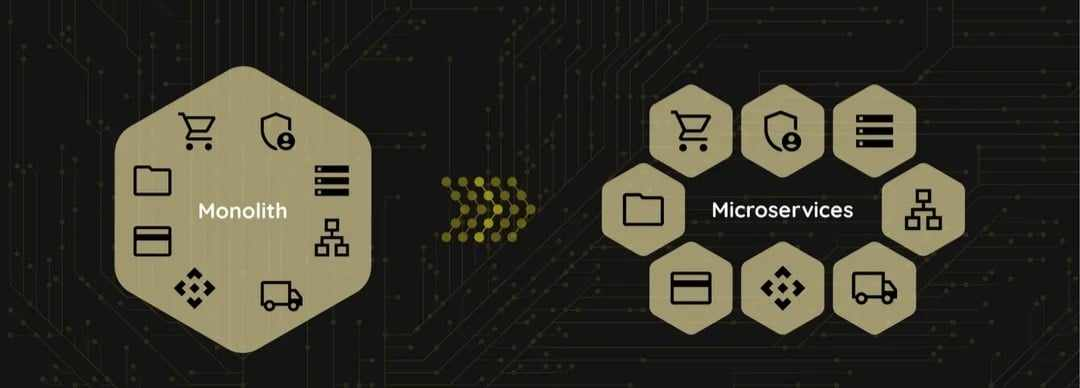
\includegraphics[height = 3cm]{pictures/ChuyenTu_KienTrucNguyenKhoi_Sang_KienTrucViDichVu.jpg}

% % \caption{ViDuHinhAnhTheoChieuDoc}

% \end{figure}

% \begin{figure}[h]

% \centering

% 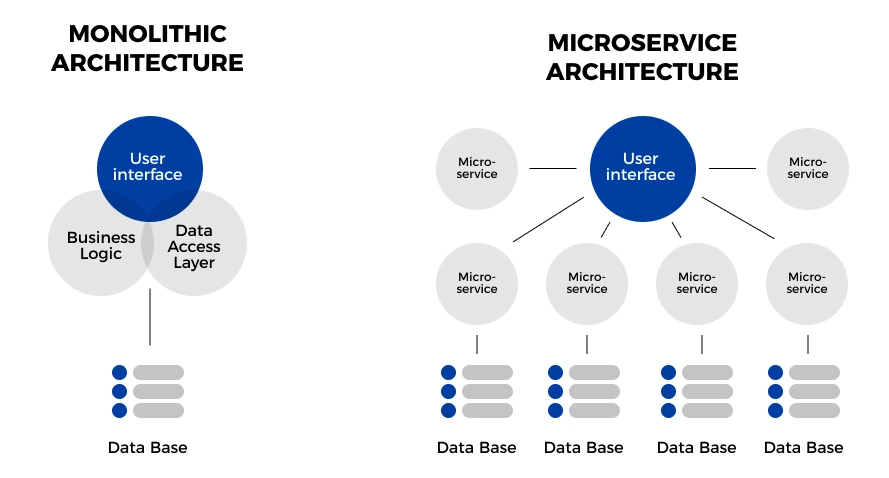
\includegraphics[height = 3cm]{pictures/AnhKhacNhau_KienTrucNguyenKhoi_KienTrucViDichVu.png}

% % \caption{ViDuHinhAnhTheoChieuDoc}

% \end{figure}

% Strangler Fig là chuyển mono sang dịch vụ

Kiến trúc kiến trúc vi dịch vụ (hay đơn giản là kiến trúc vi dịch vụ) là một cách xây dựng các ứng dụng phần mềm dưới dạng tập hợp các dịch vụ nhỏ, độc lập giao tiếp với nhau thông qua API. Mỗi dịch vụ tập trung vào một khả năng kinh doanh cụ thể và có thể được triển khai, mở rộng quy mô và duy trì độc lập với các dịch vụ khác trong hệ thống. Cách tiếp cận này nhấn mạnh tính mô - đun, tính linh hoạt và khả năng phục hồi, cho phép các nhóm làm việc đồng thời trên các phần khác nhau của hệ thống và cho phép phát hành nhanh hơn và thường xuyên hơn. Các vi dịch vụ thường dựa vào các giao thức truyền thông nhẹ, chẳng hạn như REST và thường được triển khai bằng các công nghệ chứa trong bộ chứa như Docker và Kubernetes.
